\documentclass[11pt]{beamer}
\usetheme{Boadilla}
\usepackage[utf8]{inputenc}
\usepackage[spanish]{babel}
\usepackage{amsmath}
\usepackage{amsfonts}
\usepackage{amssymb}
\usepackage{graphicx}
\usepackage{subfig}
\usepackage{natbib}

%%%%% Color institucional
\definecolor{MyBackground}{rgb}{1.0000,0.9451,0.6549}
\definecolor{itesm}{HTML}{0658a6}
\definecolor{lnppdos}{RGB}{59,124,188}
\definecolor{lnpptres}{RGB}{124,172,212}
%\definecolor{MyBackground}{RGB}{255,241,167}
%\setbeamercolor{background canvas}{bg=MyBackground}
\setbeamercolor*{palette primary}{bg=lnpptres, fg = black}
\setbeamercolor*{palette secondary}{bg=lnppdos, fg = white}
\setbeamercolor*{palette tertiary}{bg=itesm, fg = white}
\setbeamercolor{frametitle}{fg=itesm,bg=white}
\setbeamercolor{title}{fg=white,bg=itesm}
\setbeamercolor{caption name}{fg=itesm}
\setbeamercolor*{item}{fg=itesm}
\usepackage{xcolor}

%%%%%%
\title[]{Virtualización y Contenedores en Cómputo Científico}
\institute[ITESM]{Data Pub\\ ITESM} 
\date{\today} 
\subject{Resultados} 
\titlegraphic{
\includegraphics[width=3cm]{images/itesm}\hspace*{7.5cm}
}
%\title{Turing ODE}
%\setbeamercovered{transparent} 
%\setbeamertemplate{navigation symbols}{} 
%\logo{} 
%\institute{} 
%\date{} 
%\subject{} 
\begin{document}

\begin{frame}
\titlepage
\end{frame}

%\begin{frame}
%\tableofcontents
%\end{frame}

\begin{frame}{Centros de Super Cómputo}
	\begin{figure}
		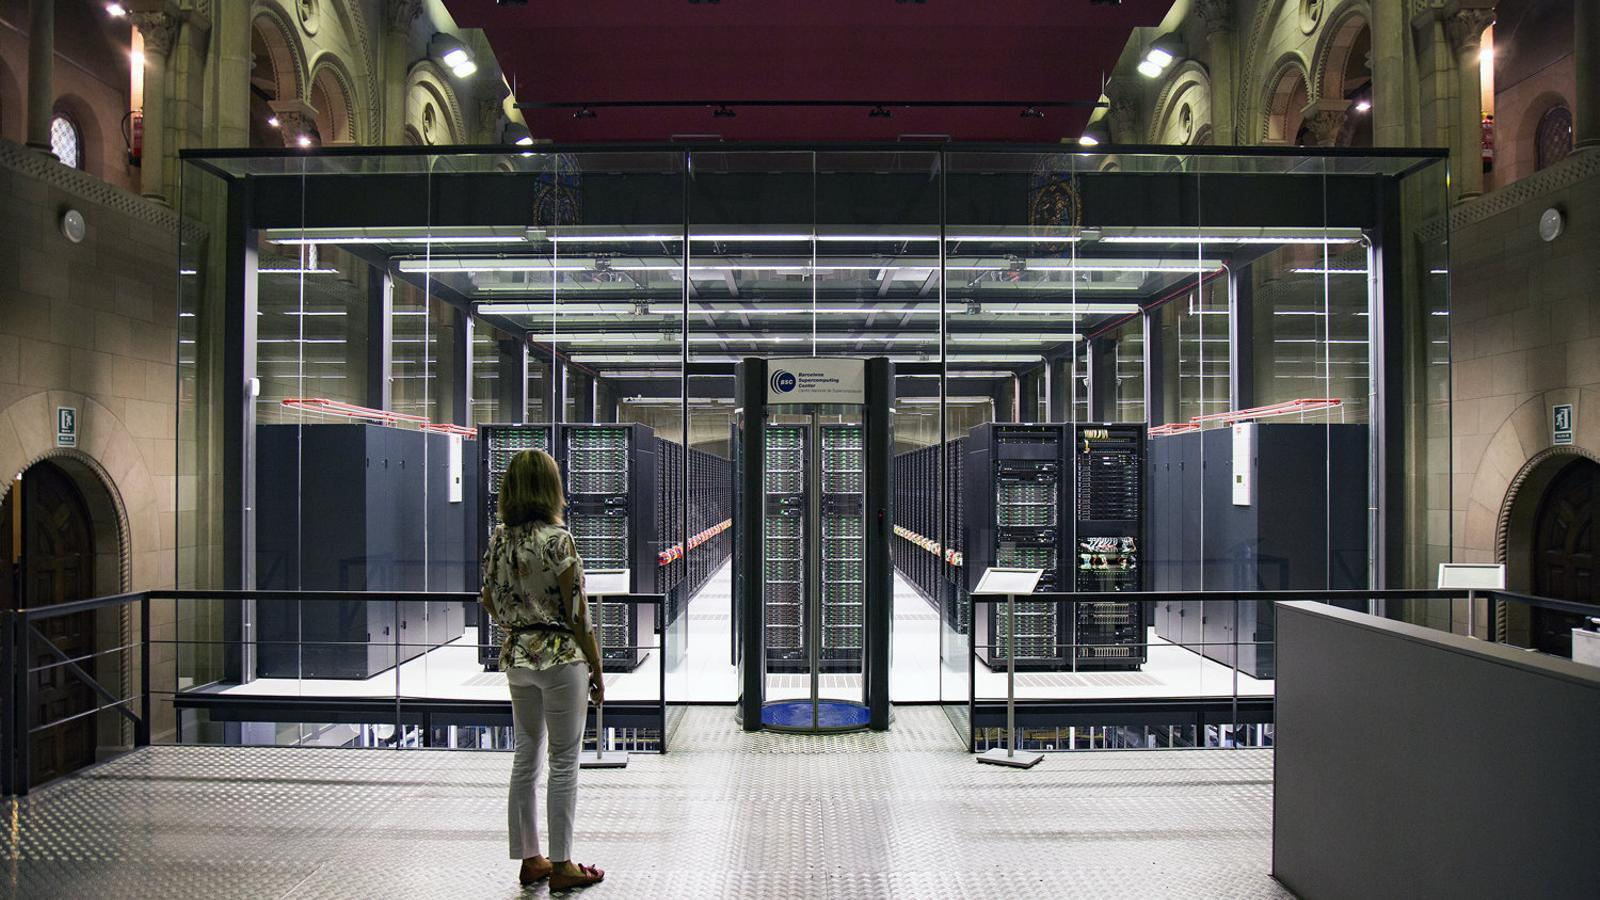
\includegraphics[scale=0.2]{images/barcelona_supercomputing.jpg}
		\caption{Barcelona Supercomputing Center}
	\end{figure}
\end{frame}

\begin{frame}{Centros de Super Cómputo}
	\begin{center}
		\textbf{Centros de Super Cómputo : Recurso compartido}
	\end{center}
	
	\begin{itemize}
		\item  \textbf{Usuaria-Clienta}. Relacionadas con un grupo o institución.
		\item \textbf{Administradoras}. Satisfacen distintas necesidades de las clientas:
			\begin{itemize}
				\item Versiones de software.
				\item Compiladores.
				\item Módulos.
				\item Sistemas de archivos.
				\item Permisos.
			\end{itemize}
		
	\end{itemize}

\end{frame}

\begin{frame}{Arquitectura de un Cluster de HPC}
	\vspace{-0.5cm}
	\begin{figure}
		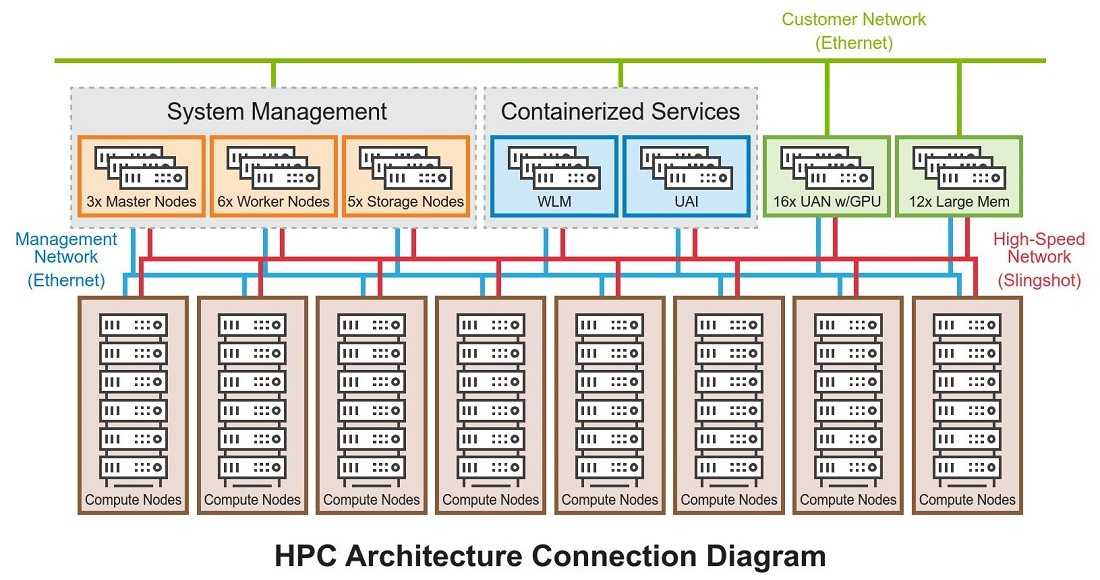
\includegraphics[scale=0.42]{images/hpc_cluster}
		\caption{Tomado de \url{https://www.gigabyte.com/Article/high-performance-computing-cluster}}
	\end{figure}
\end{frame}

\begin{frame}{¿Cómo se administra un Cluster con miles de nodos?}

\begin{columns}
\begin{column}{0.5\textwidth}
  \textbf{Herramientas de configuración automatizada}
  
  \begin{figure}
  	
\includegraphics[scale=0.3]{images/cfengine}
  	
\includegraphics[scale=0.3]{images/ansible}
  \end{figure}
\end{column}
\begin{column}{0.5\textwidth}  %%<--- here
  \textbf{Job Scheduler o Resource Management System(RMS)}
    \begin{figure}
  	
\includegraphics[scale=0.3]{images/slurm}
  	
\includegraphics[scale=0.3]{images/condor}
  \end{figure}
\end{column}
\end{columns}

\end{frame}



\begin{frame}{Dos visiones}
\begin{columns}
\begin{column}{0.5\textwidth}
  \textbf{Administradoras}
  
  Se aseguran que la clienta-usuaria tenga las herramientas y soporte necesario para el uso eficiente de los recursos.
  \begin{figure}
  	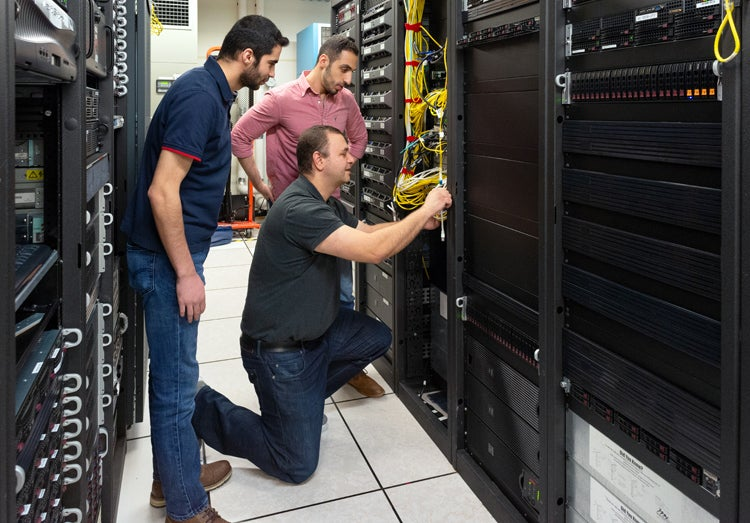
\includegraphics[scale=0.2]{images/sysadmin_humano}
  \end{figure}
\end{column}
\begin{column}{0.5\textwidth}  %%<--- here
  \textbf{Usuarias}
  
  Consume los recursos.
  \vspace{1.4cm}
    \begin{figure}
  	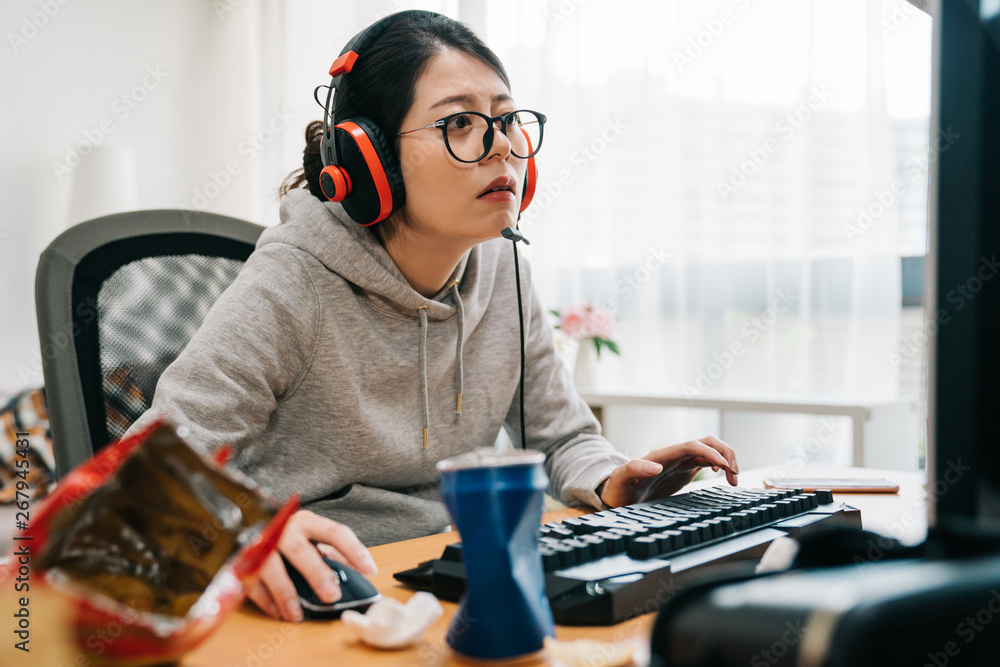
\includegraphics[scale=0.65]{images/usuario_hpc}

  \end{figure}
\end{column}
\end{columns}
\end{frame}

\begin{frame}{Todo parece estar bien ... }
	\begin{figure}
		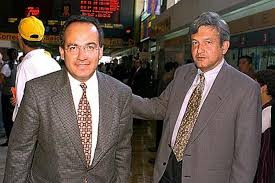
\includegraphics[scale=0.8]{images/armonia_cuatro	}
	\end{figure}
\end{frame}

\begin{frame}{La realidad es otra}
	\begin{figure}
		
\includegraphics[scale=0.3]{images/realidad}
	\end{figure}
\end{frame}


\begin{frame}{Problema}

	\begin{itemize}
		\item Como en todo aquello donde existe el uso de un recurso compartido, las relaciones Sysadmin-Usuaria, Usuaria-Usuaria no son siempre coordiales. 
		\item Hay conflicto : ¿Quién y cuándo tiene acceso al recurso?¿Hay asignación justa de recursos?¿Hay usuarios con mayores privilegios?
		\item \textbf{Sysadmin} : Definen \textbf{Reglas-Políticas de uso} con el objetivo de satisfacer las necesidades de las usuarias pero también acorde a las necesidades de mantener un recurso usable y confiable.
		\item \textbf{Usuaria} : Estas reglas y políticas se traduce en sistemas y software limitantes e inmóviles \citep{kurtzer2017singularity}. 
	\end{itemize}

\end{frame}

\begin{frame}{Problema}

	\begin{center}
		\textit{This static nature coupled with distribution-specific software builds meant that service providers would ultimately end up limiting the scope of computational science that their systems could support}\citep{kurtzer2017singularity}
	\end{center}

\end{frame}

\begin{frame}{Propuesta de solución\citep{kurtzer2017singularity}}
	\textbf{Ambientes portables}
	
	\begin{itemize}
		\item Máquinas virtuales.
		\item Contenedores.
	\end{itemize}
\end{frame}

\begin{frame}{Máquinas virtuales}

\begin{columns}
\begin{column}{0.5\textwidth}

  \begin{figure}
  	
\includegraphics[scale=0.3]{images/vmachines}
  \end{figure}
\end{column}
\begin{column}{0.5\textwidth}  %%<--- here

	Proporcionan un ambiente completo, incluyendo dependencias de software, bibliotecas, datos que pueden ser encapsulados y ejecutados donde sea.
	
	\begin{center}
		\textbf{Problema}
	\end{center}
	
Introduce una sobrecarga computacional considerable debido al nivel requerido de virtualización para emular el sistema operativo y el kernel.
\end{column}
\end{columns}
\end{frame}



\begin{frame}{Contenedores}
	\begin{columns}
\begin{column}{0.5\textwidth}

  \begin{figure}
  	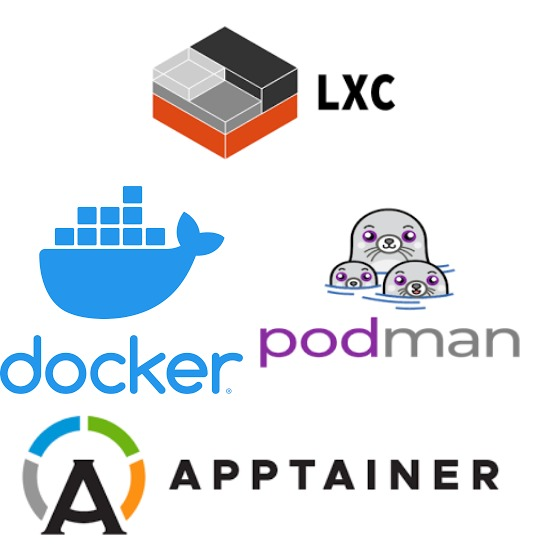
\includegraphics[scale=0.3]{images/contenedores_tecnologias}
  \end{figure}
\end{column}

	\vspace{-0.5cm}

\begin{column}{0.5\textwidth}  %%<--- here
	
	Características de virtualización ligera en el kernel de Linux hace posible construir virtualización más ligera. 

	\vspace{0.2cm}
	
	Las características específicas del kernel son las que se ocupan de aislar procesos, en particular \citep{nemeth2018unix}:
	
		\begin{itemize}
			\item \textbf{Namespaces} : aislan los procesos del contenedor desde la perspectiva de las características del sistema operativo.
			\item \textbf{Control groups (cgroups)} limita el uso de los recursos del sistema y prioriza ciertos procesos sobre otros.
					\end{itemize}

	
\end{column}
\end{columns}
\end{frame}

\begin{frame}[allowframebreaks]
        \frametitle{References}
		\bibliographystyle{apalike}

       \bibliography{apptainer_virtualizacion.bib}
\end{frame}

\end{document}